%%%%%%%%%%%%%%%%%%%%%%%%%%%%%%%%%%%%%%%%%%%%%%%%
%% Intro to LaTeX and Template for Homework Assignments
%% Quantitative Methods in Political Science
%% University of Mannheim
%% Fall 2017
%%%%%%%%%%%%%%%%%%%%%%%%%%%%%%%%%%%%%%%%%%%%%%%%

% created by Marcel Neunhoeffer & Sebastian Sternberg


% This template and tutorial will help you to write up your homework. It will also help you to use Latex for other assignments than this course's homework.

%%%%%%%%%%%%%%%%%%%%%%%%%%%%%%%%%%%%%%%%%%%%%%%%
% Before we get started
%%%%%%%%%%%%%%%%%%%%%%%%%%%%%%%%%%%%%%%%%%%%%%%%

% Make an account on overleaf.com and get started. No need to install anything.

%%%%%%%%%%%%%%%%%%%%%%%%%%%%%%%%%%%%%%%%%%%%%%%%
% Or if you want it the nerdy way...
% INSTALL LATEX: Before we can get started you need to install LaTeX on your computer.
				% Windows: http://miktex.org/download
				% Mac:         http://www.tug.org/mactex/mactex-download.html	
				% There a many more different LaTeX editors out there for both operating systems. I use TeXworks because it looks the same on Windows and Mac.
				

% SAVE THE FILE: The first thing you need to do is to save your LaTeX file in a directory as a .tex file. You will not be able to do anything else unless your file is saved. I suggest to save the .tex file in the same folder with your .R script and where you will save your plots from R to. Let's call this file template_homework1.tex and save it in your Week 1 folder.


% COMPILE THE FILE: After setting up your file, using your LaTeX editor (texmaker, texshop), you can compile your document using PDFLaTeX.
	% Compiling your file tells LaTeX to take the code you have written and create a pdf file
	% After compiling your file, in your directory will appear four new files, including a .pdf file. This is your output document.
	% It is good to compile your file regularly so that you can see how your code is translating into your document.
	
	
% ERRORS: If you get an error message, something is wrong in your code. Fix errors before they pile up!
	% As with error messages in R, google the exact error message if you have a question!
%%%%%%%%%%%%%%%%%%%%%%%%%%%%%%%%%%%%%%%%%%%%%%%%


% Now again for everyone...

% COMMANDS: 
	% To do anything in LaTeX, you must use commands
	% Commands tell LaTeX when to start your document, how you want your document to look, and how to format your document
	% Commands ALWAYS begin with a backslash \

% Everything following the % sign is a comment and will not be used by Latex to compile your document.
% This is very similar to # comments in R.

% Every .tex file usually consists of four parts.
% 1. Document Class
% 2. Packages
% 3. Header
% 4. Your Document

%%%%%%%%%%%%%%%%%%%%%%%%%%%%%%%%%%%%%%%%%%%%%%%%
% 1. Document Class
%%%%%%%%%%%%%%%%%%%%%%%%%%%%%%%%%%%%%%%%%%%%%%%%
 
 % The first command you will always have will declare your document class. This tells LaTeX what type of document you are creating (article, presentation, poster, etc). 
% \documentclass is the command
% in {} you specify the type of document
% in [] you define additional parameters
 
\documentclass[a4paper,11pt]{article} % This defines the style of your paper

% We usually use the article type. The additional parameters are the format of the paper you want to print it on and the standard font size. For us this is a4paper and 12pt.

%%%%%%%%%%%%%%%%%%%%%%%%%%%%%%%%%%%%%%%%%%%%%%%%
% 2. Packages
%%%%%%%%%%%%%%%%%%%%%%%%%%%%%%%%%%%%%%%%%%%%%%%%

% Packages are libraries of commands that LaTeX can call when compiling the document. With the specialized commands you can customize the formatting of your document.
% If the packages we call are not installed yet, TeXworks will ask you to install the necessary packages while compiling.

% First, we usually want to set the margins of our document. For this we use the package geometry. We call the package with the \usepackage command. The package goes in the {}, the parameters again go into the [].
\usepackage[top = 2cm, bottom = 2.5cm, left = 2.5cm, right = 2cm]{geometry} 

% Unfortunately, LaTeX has a hard time interpreting German Umlaute. The following two lines and packages should help. If it doesn't work for you please let me know.
\usepackage[T1]{fontenc}
\usepackage[utf8]{inputenc}

% The following two packages - multirow and booktabs - are needed to create nice looking tables.
\usepackage{multirow} % Multirow is for tables with multiple rows within one cell.
\usepackage{booktabs} % For even nicer tables.

% As we usually want to include some plots (.pdf files) we need a package for that.
\usepackage{graphicx} 

% The default setting of LaTeX is to indent new paragraphs. This is useful for articles. But not really nice for homework problem sets. The following command sets the indent to 0.
\usepackage{setspace}
\setlength{\parindent}{0in}
\setlength{\parskip}{0.25em}
% Package to place figures where you want them.
\usepackage{float}
\usepackage{minted}
% The fancyhdr package let's us create nice headers.
\usepackage{fancyhdr}

\usepackage{amsmath,amssymb}
\usepackage{xcolor}
\usepackage{hyperref}
\hypersetup{
    colorlinks=true,
    linkcolor=blue,
    filecolor=magenta,      
    urlcolor=cyan,
}
\usepackage{soul} % for highlighting
\usepackage{graphicx} % graphics package
\usepackage{caption}
\usepackage{subcaption} % subplot package
\graphicspath{{images/}} % declare the path where graphic files are
\DeclareGraphicsExtensions{.pdf,.jpg,.png} % grafic files extensions
\usepackage{epstopdf} % package to include eps. files
\usepackage{float}
\usepackage{booktabs}
\usepackage{array}
\usepackage[linesnumbered, ruled]{algorithm2e}

\usepackage{mdframed}
\soulregister\ref7
\soulregister\cite7
\soulregister\url7
\newcommand{\highlight}[1]{\colorbox{yellow}{$\displaystyle#1$}}

%%%%%%%%%%%%%%%%%%%%%%%%%%%%%%%%%%%%%%%%%%%%%%%%
% 3. Header (and Footer)
%%%%%%%%%%%%%%%%%%%%%%%%%%%%%%%%%%%%%%%%%%%%%%%%

% To make our document nice we want a header and number the pages in the footer.



\pagestyle{fancy} % With this command we can customize the header style.

\fancyhf{} % This makes sure we do not have other information in our header or footer.

\lhead{\footnotesize \assType\ \exeNum}% \lhead puts text in the top left corner. \footnotesize sets our font to a smaller size.

%\rhead works just like \lhead (you can also use \chead)
\rhead{\footnotesize \studentName\ (\studentNumber)} %<---- Fill in your lastnames.

% Similar commands work for the footer (\lfoot, \cfoot and \rfoot).
% We want to put our page number in the center.
\cfoot{\footnotesize \thepage} 

%----------------------------------------------------------------------------------------
%	WORK EXPERIENCE FORMATTING
%----------------------------------------------------------------------------------------
% set line spacing
\newcommand{\lineSpace}{1.1}

% syntax: \newenvironment{name}{begin command}{endcommand}
\newcounter{rSection}
\newcounter{rSubsection}[rSection]

\newenvironment{rSection}[1]{ % 1 input argument - section name
\refstepcounter{rSection}
\begin{spacing}{\lineSpace}
  {\bf \large \therSection~#1 \hfill}  % Section title DO NOT delete the following blank line
	\vspace{0.25em}

}{
\vspace{1em}
\end{spacing}
}

\newenvironment{rSubsection}[1]{ % 1 input argument - section name
  \refstepcounter{rSubsection}
  \begin{spacing}{\lineSpace}
	{\bf\therSection.\therSubsection~#1}

  }{
\end{spacing}
\vspace{0.5em}
}


\newenvironment{rlisting}{
  \vspace{-0.5em}
  \begin{itemize}
	\itemsep -0.25em \vspace{-0.5em}
}{
	\vspace{-0.5em}
\end{itemize}
\vspace{-0.5em}
}

\newenvironment{renum}{
	\vspace{-0.5em}
  \begin{enumerate}
	\itemsep -0.25em \vspace{-0.5em}
}{
	\vspace{-0.5em}
\end{enumerate}
\vspace{-0.5em}
}

\definecolor{bg}{rgb}{0.95,0.95,0.95}
\renewcommand\refname{\large References}
%%%%%%%%%%%%%%%%%%%%%%%%%%%%%%%%%%%%%%%%%%%%%%%%
% 4. Your document
%%%%%%%%%%%%%%%%%%%%%%%%%%%%%%%%%%%%%%%%%%%%%%%%

% Now, you need to tell LaTeX where your document starts. We do this with the \begin{document} command.
% Like brackets every \begin{} command needs a corresponding \end{} command. We come back to this later.

%%%%%%%%%%%%%%%%%%%%%%%%%%%%%%%%%%%%%%%%%%%%%%%%%%%%%%
\newcommand{\exeNum}{}
\newcommand{\assType}{Comparing Collaborative Filtering and Neural Network in Movie Recommender System}
\newcommand{\courseName}{CS-C3240 Machine Learning}
\newcommand{\semester}{Spring 2021}
\newcommand{\studentName}{Weijiang Xiong}
\newcommand{\studentNumber}{875581}
%%%%%%%%%%%%%%%%%%%%%%%%%%%%%%%%%%%%%%%%%%%%%%%%%%%%%%
\begin{document}
\linespread{\lineSpace} % line spacing

%%%%%%%%%%%%%%%%%%%%%%%%%%%%%%%%%%%%%%%%%%%%%%%%
%%%%%%%%%%%%%%%%%%%%%%%%%%%%%%%%%%%%%%%%%%%%%%%%

%%%%%%%%%%%%%%%%%%%%%%%%%%%%%%%%%%%%%%%%%%%%%%%%
% Title section of the document
%%%%%%%%%%%%%%%%%%%%%%%%%%%%%%%%%%%%%%%%%%%%%%%%

% For the title section we want to reproduce the title section of the Problem Set and add your names.

\thispagestyle{empty} % This command disables the header on the first page. 

\begin{tabular}{p{15.5cm}} % This is a simple tabular environment to align your text nicely 
{\large \bf \courseName \hfill \semester} \\
\hline % \hline produces horizontal lines.
\\
\end{tabular} % Our tabular environment ends here.

% \vspace{0.3cm} % Now we want to add some vertical space in between the line and our title.

\begin{center} % Everything within the center environment is centered.
	{\Large \bf \assType\ \exeNum} % <---- Don't forget to put in the right number

	{\studentName\ (Student Number \studentNumber)} % <---- Fill in your names here!
		
\end{center}  
% 

%%%%%%%%%%%%%%%%%%%%%%%%%%%%%%%%%%%%%%%%%%%%%%%%
%%%%%%%%%%%%%%%%%%%%%%%%%%%%%%%%%%%%%%%%%%%%%%%%

% Up until this point you only have to make minor changes for every week (Number of the homework). Your write up essentially starts here.

\begin{rSection}{Introduction}
	Recommender systems are widely used in our daily life. 
	Whenever we open a shopping website like Amazon, or a video website like YouTube, we would see a bunch of items in the front page.
	Those items are generated by a recommender system, which infers our preferences based on our activities, such as browsing history, ratings and purchases. 
	A good recommender system would suggest good contents that we would like to see, and thus will make our life more convenient.
	
	This project report will briefly introduce how to build a recommender system for movies.
	Section \ref{sec: problem formulation} presents how the problem is formulated.
	Section \ref{sec: methods} elaborates on two methods, namely collaborative filtering and neural networks.
	Section \ref{sec: experiments and results} shows the results from experiments.
	Finally, Section \ref{sec: conclusions} draws a conclusion and summarizes the whole report.

	% \begin{rSubsection}{The first part of the problem}
	% 	in the first subsection, build a list with \mintinline{latex}{\begin{rlisting}}
	% 	\begin{rlisting}
	% 		\item just write something random
	% 		\item another random line
	% 	\end{rlisting}
	% 	build an ordered list with \mintinline{latex}{\begin{renum}}
	% 		\begin{renum}
	% 			\item just write something random
	% 			\item another random line
	% 		\end{renum}
	% \end{rSubsection}

	% \begin{rSubsection}{The second part of the problem}
	% 	in the second subsection, insert a figure
	% 	\begin{figure}[H]
	% 		\centering
	% 		\includegraphics[width=0.45\textwidth]{example-image-a}
	% 		\caption{Add captions here}
	% 	\end{figure}

	% 	Two figures with individual numbering and caption. Comment out \mintinline{text}{\caption{}} to remove individual caption for subfigures.
	% 	\begin{figure}[H]
	% 		\centering
	% 		\begin{subfigure}[t]{0.45\textwidth}
	% 		  \centering	
	% 		  \includegraphics[width=\textwidth]{example-image-a}
	% 		  \caption{some comments on this figure}
	% 		\end{subfigure}
	% 		\qquad
	% 		\begin{subfigure}[t]{0.45\textwidth}
	% 		  \includegraphics[width=\textwidth]{example-image-a}
	% 		  \caption{some other comments}
	% 		\end{subfigure}
	% 		\caption{Geometrical figures}
	% 	  \end{figure}
		
	% 	Text with picture left-right structure, remember to keep the blank line below (maybe not very useful)

	% 	\begin{figure}[H]
	% 		\begin{minipage}[b]{0.5\linewidth} % use [c] here makes the text vertically centered
	% 			\centering
	% 			\includegraphics[width=\textwidth]{example-image-a}
	% 			\caption{some comments}
	% 		\end{minipage}%
	% 		\begin{minipage}[b]{0.5\linewidth} % use [c] here makes the text vertically centered
	% 			\centering
	% 			\begin{tabular}{|c|c|} 
	% 				\hline
	% 				aa & bb \\ \hline
	% 				cc & dd \\ \hline
	% 			\end{tabular}
	% 			\captionof{table}{Table caption}
	% 		\end{minipage}
	% 	\end{figure}

	% 	Maybe you need to cite something \cite{danelljan2014BMVC}, and you can specify the IEEE style by using in the end \mintinline{text}{\bibliographystyle{ieee_fullname}}, Elsevier Style with \mintinline{text}{elsarticle-num} and Harvard Style with \mintinline{text}{elsarticle-harv0}.
	% 	After this, please compile the tex file with \mintinline{text}{pdflatex->bibtex->pdflatex->pdflatex}.
	% 	If the main text has not cited anything, just use \mintinline{text}{pdflatex}
	% \end{rSubsection}

\end{rSection}


\begin{rSection}{Dataset and Problem Description}
\label{sec: problem formulation}
According to the textbook \cite{MLBook}, a machine learning problem consists of three parts: data, model and loss.
Now we will discuss the data part here and leave model and loss to Section \ref{sec: methods}.
This methods in this report will be built with the Movie Lens Dataset \cite{MovieDataset} by Grouplens Research.
This dataset contains 100835 ratings of 9724 movies from 610 people, and the ratings range from 0 to 5 with a step at 0.5.
The following table shows the first three rows of the entire dataset.

\begin{table}[H]
	\centering
	\caption{Entries in Movie Lens Dataset}
	\begin{tabular}{c|cccc}
		\toprule
		& User ID & Movie ID & Rating  \\
		\midrule
		1 & 1 & 3& 4.0 \\
		2 & 1 & 6 &4.0\\
		3 & 1 & 47 & 5.0 \\
		\vdots & \vdots &\vdots &\vdots\\
		\bottomrule
	\end{tabular}
\end{table}

In this problem, a \textbf{data point} is a row in the table, which is a tuple with elements User ID, Movie ID and Rating.
User ID and Movie ID serve as \textbf{features}, and Rating will be considered as \textbf{label}.
Specifically in this dataset, User ID is an integer ranging from 1 to 610 without, but Movie ID ranges from 1 to 193609 and is not continuous.
Concretely, the task of a recommender system is to predict a user's rating (unknown) of a movie, given a set of records (User ID, Movie ID and Rating).
And we will see how to build such a system in the following section. 

% \begin{rSubsection}{the first step}
% 	this is for inserting codes with or without a bounding box, remember to use \mintinline{text}{PDFLaTeX}

% 	\begin{minted}[bgcolor=bg,autogobble]{python}
% 		import numpy as np
% 		def some_function(some_variables):
% 			pass
% 	  \end{minted}
% 	You will need to explain the codes a bit.

% 	\begin{mdframed}[backgroundcolor=bg]
% 	\begin{minted}[autogobble,tabsize=4]{python}
% 		import numpy as np
% 		def some_function(some_variables):
% 			pass
% 	\end{minted}
% 	\end{mdframed}
% 	You will need to explain the codes a bit.
% \end{rSubsection}

% \begin{rSubsection}{the second step}
% 	We may need to type matrix equations 
% 	\begin{equation}
% 		T = 
% 		\left[\begin{matrix} m_u & 0 & 0 \\0 & m_v & 0 \\ 0 & 0 & 1 \end{matrix}\right]
% 		\left[\begin{matrix} 1 & 0 & u_{0} \\0 & 1 & v_{0} \\ 0 & 0 & 1 \end{matrix}\right]
% 		\left[\begin{matrix} f & 0 & 0 \\0 & f & 0 \\ 0 & 0 & 1 \end{matrix}\right]
% 		=
% 		\left[\begin{matrix} fm_u & 0 & u_0 \\0 & fm_v & v_0 \\ 0 & 0 & 1 \end{matrix}\right].
% 	\end{equation}
% 	If you don't want the auto numbering 
% 	$$
% 		T = \left[\begin{matrix} m_u & 0 & 0 \\0 & m_v & 0 \\ 0 & 0 & 1 \end{matrix}\right]
% 		\left[\begin{matrix} 1 & 0 & u_{0} \\0 & 1 & v_{0} \\ 0 & 0 & 1 \end{matrix}\right]
% 		\left[\begin{matrix} f & 0 & 0 \\0 & f & 0 \\ 0 & 0 & 1 \end{matrix}\right]
% 		=
% 		\left[\begin{matrix} fm_u & 0 & u_0 \\0 & fm_v & v_0 \\ 0 & 0 & 1 \end{matrix}\right].
% 	$$
% 	or build a table to present data
% 	\begin{table}[H]
% 		\centering
% 		\caption{Some random numbers}
% 		\begin{tabular}{c|cccc}
% 			\toprule
% 			($\alpha$, $u$)& 0.7 & 0.8 & 0.9 & 1 \\
% 			\midrule
% 			1 & 25.3183 & 25.5442& 25.7192& 25.8589 \\
% 			2 & 36.8104 & 37.6098 &38.2343 & 38.7359\\
% 			3 & 44.1152 & 46.6144 & 48.6152 & {50.2597} \\
% 			4 & 39.3190& 44.5661&\textcolor{red}{48.3255} &\textcolor{red}{51.3635} \\
% 			5 & 18.0562& 35.4232 &42.3844 &47.0238 \\
% 			\bottomrule
% 		\end{tabular}
% 	\end{table}
% \end{rSubsection}
\end{rSection}

\begin{rSection}{Methods}
\label{sec: methods}
In this section, we discuss two methods for a recommender system. 
The first one is called Collaborative Filtering, which was introduced in Round 3 by Prof. Stephan Sigg~\cite{RSLecture}.
The second is a feed forward neural network, which is implemented with PyTorch.
Notably, this network contains an embedding layer~\cite{embedding} and the network structure is inspired by Lecture 4 in CS-E4890 Deep Learning~\cite{DLCourse}, as well as the corresponding assignment.

In the Collaborative Filtering model, the estimated rating $\hat{r}_{u i}$ of movie $i$ from user $u$ is a biased inner product of the item (movie) vector $q_i$ and user vector $p_u$:
\begin{equation}
	\hat{r}_{u i}=\mu+b_{u}+b_{i}+q_{i}^{T} p_{u},
\end{equation}
where $\mu$ denotes the average rating of all movies, and $b_{u}$ and $b_{i}$ stands for user and item biases.
Meanwhile, the vector representations of users and items as well as their biases can be learned jointly, by minimizing a \textbf{regularized mean square error} function:
\begin{equation}
	\label{equ: reg mse loss}
	\sum_{r_{u i} \in Trainset}
	\left(r_{u i}-\hat{r}_{u i}\right)^{2}+
	\lambda\left(b_{i}^{2}+b_{u}^{2}+\left\|q_{i}\right\|^{2}+\left\|p_{u}\right\|^{2}\right),
\end{equation}
where $r_{ui}$ means the true rating of movie $i$ given by user $u$.
As stated in the lecture~\cite{RSLecture}, it's hard to optimize $q_i$ and $p_u$ simultaneously, but we can optimize them alternatively using gradient descent.
Notably, this report implements collaborative filtering with the python package \mintinline{text}{Surprise}~\cite{surprise}.

The embedding neural network is implemented with the following codes. 
The two embedding layers map the original user ID and item ID to vectors with length \mintinline{text}{n_embed}, and then these embedded features will be fed to the \mintinline{text}{hidden_block}, which uses the \mintinline{text}{Tanh} function for activation.
Finally, the hidden features will be processed by a linear output layer.
Similar to collaborative filtering, we use a \textbf{mean square error} for this neural network, which is just the first term in Equation (\ref{equ: reg mse loss}).
The loss function will be implemented with \mintinline{text}{torch.nn.MSELoss}, and we apply \mintinline{text}{Dropout}~\cite{hinton2012dropout} for regularization. 

\begin{minted}[bgcolor=bg,autogobble]{python}
import torch 
import torch.nn as nn
class RecommenderSystem(nn.Module):
    def __init__(self, n_users, n_items, n_embed=40, 
		dropout_rate=0.2, hidden_neurons=[10]):
        super(RecommenderSystem, self).__init__()
        self.user_emb = nn.Embedding(n_users, n_embed)
        self.item_emb = nn.Embedding(n_items, n_embed)
        hidden_block = []
        last_output = n_embed*2
        for n_hidden in hidden_neurons:
            hidden_block.append(nn.Linear(last_output, n_hidden))
            hidden_block.append(nn.Tanh())
            hidden_block.append(nn.Dropout(p=dropout_rate))
            last_output = n_hidden
        self.hidden_block = nn.Sequential(*hidden_block)
        del hidden_block
        self.output_layer = nn.Linear(last_output, 1)
        
    def forward(self, user_ids, item_ids):
        user_feat = self.user_emb(user_ids-1)
        item_feat = self.item_emb(item_ids-1)
        x = torch.cat([user_feat, item_feat], dim=1)
        x = self.hidden_block(x)
        x = self.output_layer(x)
        return torch.squeeze(x)
\end{minted}

There are two reason for using (regularized) MSE Loss for both of the methods.
First, MSE Loss is a continuous function, and therefore easy to apply gradient based optimization.
Second, MSE Loss penalize high deviation heavily, this allows us to obtain results that are close to true value.

\end{rSection}


\begin{rSection}{Experiments and Results}
Before any of the following experiments, we need to reserve a part of data for the final test, and use the other data for training and validation.
Specifically, the size of training, validation and testing data are 60\%, 20\% and 20\%.
To do this, we need to load the original data table, shuffle the data and then save 20\% to a file for final testing.
After that, we save the rest 80\% and proceed with "training-testing" scheme. 
For the complete code of this project report, please refer to this link \url{https://github.com/Weijiang-Xiong/CS-C3240-Project}.
\label{sec: experiments and results}

\begin{rSubsection}{Collaborative Filter}
To construct a suitable dataset for the algorithm, we need to use the built in classes \mintinline{text}{Dataset} and \mintinline{text}{Reader} in the \mintinline{text}{Surprise} package.

\begin{minted}[bgcolor=bg,autogobble]{python}
# timestamps are recorded but we don't need them
cols = ['user_ids', 'item_ids', 'ratings', 'timestamps'] 
data = pd.read_csv(data_dir + "/" +"ratings_train_valid.csv", names=cols, header=1)
dataset = Dataset.load_from_df(data[['user_ids', 'item_ids', 'ratings']], Reader())
\end{minted}

After that, the implementation of Collaborative Filter can be done in a few lines of codes with the \mintinline{text}{SVD} method~\cite{SVD} .
The following code block briefly shows the key computations done for the evaluation, the related \mintinline{text}{import} statements are omitted here.

\begin{minted}[bgcolor=bg,autogobble]{python}
def compute_mse(pred, label):
    pred, ref = np.array(pred), np.array(label)
    return np.mean((pred-ref)**2)

def pred_results(algo, testset):
    output = algo.test(testset)
    preds = [x.est for x in output]
    labels = [x.r_ui for x in output]
    return preds, labels
# test_size is 0.25 because we need 20% data for validation, but the file 
# contains 80% of the whole data, 0.8*0.25 = 0.2
trainset, validset = train_test_split(dataset, test_size=0.25, shuffle=True)
train_preds, train_labels = pred_results(svd.fit(trainset), trainset.build_testset())
print("MSE on Train Set {}".format(compute_mse(train_preds, train_labels)))
valid_preds, valid_labels = pred_results(svd, validset)
print("MSE on Validation Set {}".format(compute_mse(valid_preds, valid_labels)))
\end{minted}

The training set and validation set are obtained by a single random split, where the validation set takes 20\% of the whole dataset.
This split is done with the \mintinline{text}{train_test_split} function in \mintinline{text}{Surpirse} package, and it works like the split function in \mintinline{text}{sklearn}.
Here, the training and validation process could be simply done by \mintinline{text}{fit} and \mintinline{text}{test}.
After some hyperparameter tuning, the hyperparameter set that gives the lowest MSE error on \mintinline{text}{testset} has been adopted to produce the final result.
In this case, the MSE loss on \mintinline{text}{trainset} is 0.64, and that for \mintinline{text}{testset} is 0.77.
Since the training loss is not significantly lower than the test loss, it's reasonable to say the model has not over-fit too much.
\end{rSubsection}

\begin{rSubsection}{Embedding Net}
The Embedding Net \mintinline{text}{RecommenderSystem} is implemented with PyTorch, and the optimizer for the training process is the \mintinline{text}{Adam} optimizer in \mintinline{text}{torch.optim}.
Since a single data point is small, we can feed a large batch each time and choose a larger learning rate.
For this report, the batch size is chosen at 1024 and learning rate 0.01.
The whole training process consists of 30 epochs, and in each epoch, we record the training loss and validation loss, which are presented in the figure below.

While the implementation of collaborative filter needs just a few lines of codes, training a neural net actually requires more work. 
Please refer to the github repo for the complete code.
\begin{figure}[H]
	\centering
	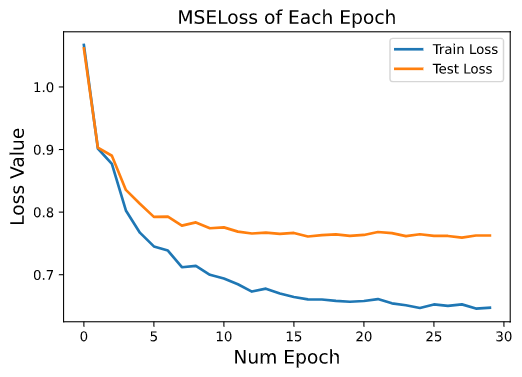
\includegraphics[width=0.6\textwidth]{loss_curve.png}
	\caption{Add captions here}
\end{figure}

This neural network achieves a best validation loss at 0.76, which is slightly lower than the collaborative filter implementation.
Therefore, for this movie recommender system, we would prefer the Embedding net solution.
Further, we test the trained neural net with the initially reserved test set, and final test error turns out to be 0.76, which is almost the same as the validation loss.
\end{rSubsection}
\end{rSection}


\begin{rSection}{Conclusions}
\label{sec: conclusions}
In this project, we've seen how to build a recommender system by collaborative filtering and embedding neural network.
According to the experiment results, the validation loss of collaborative filter is 0.76, compared to 0.77 of the embedding net.
Although we prefer the neural net solution, we can not yet certainly conclude it is better than the filtering solution.
The validation loss and final testing loss of the neural net are fairly close, and both of them are approximately 0.1 higher than training loss.
The neural net is prone to over-fit, and therefore a good direction for future work is to test these two kinds of solutions on larger dataset.
\end{rSection}

\clearpage

\bibliographystyle{ieee_fullname}
% \bibliographystyle{elsarticle-num}
% \bibliographystyle{elsarticle-harv}
\bibliography{EXAMPLE_BIB}

\clearpage

\end{document}
